\documentclass[12pt, a4paper]{article}

\usepackage{amsmath}
\usepackage{array}
\usepackage{amsmath}
\usepackage[portuguese]{babel}
\usepackage{chngpage}
\usepackage{float}
\usepackage[a4paper, margin=2cm]{geometry}
\usepackage{graphicx}
\usepackage{hyperref}
\usepackage{listings}
\usepackage{setspace}
\usepackage{xcolor}

\lstdefinestyle{codestyle}{
    commentstyle=\color{teal},
    keywordstyle=\color{blue},
    numberstyle=\ttfamily\color{gray},
    stringstyle=\color{red},
    basicstyle=\ttfamily\footnotesize,
    breakatwhitespace=false,
    breaklines=false,
    keepspaces=true,
    numbers=none,
    showspaces=false,
    showstringspaces=false,
    showtabs=false,
    tabsize=4
}
\lstset{style=codestyle}

\title{\Huge \textbf{Computação Gráfica \\ \Large Trabalho Prático -- Fase II}}
\date{30 de março 2025}
\author{Grupo 3}

\begin{document}

\begin{center}
    
\includegraphics[width=0.25\textwidth]{res/cover/EE-C.eps}
\end{center}

\chardef\_=`_
\onehalfspacing
\setlength{\parskip}{\baselineskip}
\setlength{\parindent}{0pt}
\def\arraystretch{1.5}

{\let\newpage\relax\maketitle}
\maketitle
\thispagestyle{empty}

\vspace*{\fill}

\begin{adjustwidth}{-2cm}{-2cm} % These values only need to be large enough to center the table
    \begin{center}
        \begin{tabular}{>{\centering}p{0.25\textwidth}
                        >{\centering}p{0.25\textwidth}
                        >{\centering}p{0.25\textwidth}
                        >{\centering\arraybackslash}p{0.25\textwidth}}
            
\includegraphics[width=3.5cm]{res/cover/A104437.png} &
            
\includegraphics[width=3.5cm]{res/cover/A104348.png} &
            
\includegraphics[width=3.5cm]{res/cover/A90817.png} &
            
\includegraphics[width=3.5cm]{res/cover/A104179.png} \\

            Ana Oliveira & Humberto Gomes & Mariana Cristino & Sara Lopes \\
            A104437      & A104348        & A90817           & A104179
        \end{tabular}
    \end{center}
\end{adjustwidth}

\pagebreak

\begin{abstract}
    \textbf{\color{red} TODO - resumo}
\end{abstract}

\section{Transformações}

\textbf{\color{red} TODO - transformações}

\section{Modelo estático do sistema solar}

\textbf{\color{red} TODO - sistema solar}

\section{Extras}

\subsection{Roda Dentada}

A roda dentada é uma derivaçaão do cilindro, na medida em que possui uma estrutura básica
cilíndrica, no entanto tem o complemento dos dentes no exterior e uma coroa no interior. A
construção desta primitiva tem por base coordenadas cilíndricas, onde a posição de cada ponto é
dada pelo raio interno ($r_i$), raio externo ($r_e$), ângulo azimutal ($\phi$) e altura ($h$).

A parametrização de um ponto sobre uma roda dentada de raio \( r \) pode ser definida
pelas seguintes equações:

$$x = r \cos(\phi)$$
$$y \in \left [ 0, h \right ]$$
$$z =  r \sin(\phi)$$


onde $r$ possui dois valores distintos. Para a parte interna da roda é utilizado o $r_i$ e para a
parte externa o $r_e$. Os dentes são gerados na circunferência exterior, com o aumento do raio em
determinadas posições.

\subsubsection{Geração dos Vértices}

Para discretizar a superfície da roda dentada, divide-se o intervalo de $\phi$ em \emph{slices}, e
o intervalo de $y$ em \emph{stacks}. Assim, as incrementações angulares são calculadas da seguinte
forma:

$$
\Delta \phi = \frac{2\pi}{N_\text{slices}}
\hspace{1cm}
\Delta y = \frac{h}{N_\text{stacks}}
$$

A construção dos vértices segue os seguintes passos:

1. Superfície lateral externa: Para cada \emph{stack}, os valores de $\phi$ são iterados,
determinando a posição dos pontos ao longo da circunferência externa. Nos intervalos correspondentes
aos dentes, o raio é aumentado em $r_e + h_t$, onde $h_t$ é a altura do dente.

2. Superfície lateral interna: De forma similar à superfície lateral externa, é gerada a superfície
interna do cilindro, mas o raio mantém-se constante em $r_i$.

\subsubsection{Construção das Faces}

Após a geração dos vértices, é necessário definir as faces triangulares que compõem a roda dentada.
A triangulação é realizada da seguinte forma:

1. Superfície lateral externa: Os pontos adjacentes de duas \emph{stacks} consecutivas são
ligados, isto forma quadriláteros que são divididos individualmente em dois triângulos.

2. Superfície lateral interna: É aplicada a mesma estratégia ao cilindro interno, com a ligação
dos pontos entre diferentes \emph{stacks}.

3. Bases superior e inferior: Os pontos da última \emph{stack} são ligados ao vértice central
correspondente, de modo a formar triângulos radiais.

\begin{figure}[H]
    \centering
    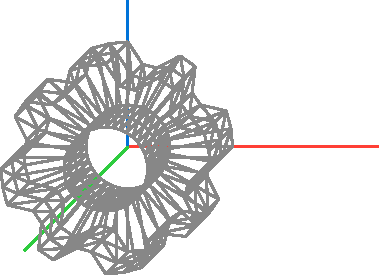
\includegraphics[width=0.3\textwidth]{res/phase2/figures/gear.pdf}
    \caption{Representação da estrutura da roda dentada.}
\end{figure}

\section{Resultados obtidos}

\textbf{\color{red} TODO - resultados}

\section{Conclusão e Trabalho Futuro}

\textbf{\color{red} TODO - conclusão}

\begingroup
\section{Bibliografia}
\renewcommand{\section}[2]{}

\begin{thebibliography}{9}
    \bibitem{exemplo}
        \href{https://youtu.be/dQw4w9WgXcQ}{Um item de exemplo na bibliografia}
\end{thebibliography}
\endgroup

\end{document}
